%==================== PARTE 2 ====================
\section{Método de simulação em malha fechada (comum aos itens)}
\subsection{Estrutura do PID (PI\_D paralelo do OpenPLC)}
\begin{formula}
$\displaystyle U(s)=\Big(K_p+\frac{K_i}{s}\Big)\big(R(s)-Y(s)\big)-D(s)\,Y(s),\qquad D(s)=\frac{K_d\,s}{\mu T_d\,s+1},\qquad K_i=\frac{K_p}{T_i},\ K_d=K_pT_d .$
\end{formula}
Aqui $R=SP$, $Y=VP$, $U=SC$ (sinal de controle). \begin{just}A ação proporcional e a integral atuam sobre o erro $e=SP-VP$; a derivada atua \emph{só sobre a VP} (e não sobre o erro) para não derivar os degraus do SP (``chute derivativo''). O filtro de constante $\mu T_d$ ($\mu=0{,}1$) limita o ganho do termo derivativo em alta frequência a $K_p(1+1/\mu)$ (a derivada pura amplificaria o ruído do ADC). É essa a implementação do OpenPLC citada no enunciado.\end{just}

\subsection{Funções de transferência de malha fechada}
Sendo $Y=GU$ e $PI(s)=K_p+K_i/s$:
\[
U=PI\,R-(PI+D)\,Y=PI\,R-(PI+D)\,G\,U\ \Rightarrow\ U\,[1+(PI+D)G]=PI\,R .
\]
\begin{res}
\[
\frac{U}{R}=\frac{PI}{1+(PI+D)G},\qquad \frac{Y}{R}=\frac{PI\,G}{1+(PI+D)G}.
\]
\end{res}
\textbf{Forma polinomial (para simular).} Escrevo $G=N_G/D_G$, $PI=(K_ps+K_i)/s$ e $D=K_ds/(\mu T_ds+1)$. Levando ao denominador comum $s(\mu T_ds+1)$:
\[\begin{gathered}
PI+D=\frac{(K_ps+K_i)(\mu T_ds+1)+K_ds^2}{s(\mu T_ds+1)}=\frac{C_n}{C_d},\\ C_n=(K_ps+K_i)(\mu T_ds+1)+K_ds^2,\ C_d=s(\mu T_ds+1).
\end{gathered}\]
Substituindo e simplificando (o fator $s$ de $C_d$ cancela com o $s$ do $PI$):
\[
\frac{Y}{R}=\frac{(K_ps+K_i)(\mu T_ds+1)\,N_G}{C_dD_G+C_nN_G},\qquad
\frac{U}{R}=\frac{(K_ps+K_i)(\mu T_ds+1)\,D_G}{C_dD_G+C_nN_G}.
\]
O denominador $C_dD_G+C_nN_G$ é o polinômio característico da malha fechada: seus polos dizem se a malha é estável. Simulo com a rotina \texttt{lsim} (a mesma do script do professor no MATLAB).

\subsection{Planta nas simulações e atraso por Padé}
Uso duas plantas $\Vc3/\Vin$: \textbf{(a) FT reduzida (FOPDT)} (eq.~\eqref{ft3} reduzida: $K=0{,}3918$, $\tau=78{,}03$, $t_0=25{,}92$) e \textbf{(b) FT completa}, eq.~\eqref{ft3}.
\begin{formula}Aproximação de Padé de ordem $n/n$ de $e^{-x}$: $\displaystyle e^{-x}\approx\frac{\sum_{k=0}^{n}(-1)^kc_kx^k}{\sum_{k=0}^{n}c_kx^k}$, $\ c_k=\frac{(2n-k)!\,n!}{(2n)!\,k!\,(n-k)!}$.\end{formula}
\begin{just}O atraso $e^{-t_0s}$ não é uma função racional, e \texttt{lsim} trabalha com polinômios. Com $t_0=25{,}92$ s, o Padé de 1ª ordem (usado no script do professor) distorce bastante; uso a de 3ª ordem ($n=3$).\end{just}
Para $n=3$: $c_0=1$; $c_1=\frac{5!\,3!}{6!\,1!\,2!}=\frac{720}{1440}=\frac12$; $c_2=\frac{4!\,3!}{6!\,2!\,1!}=\frac{144}{1440}=\frac1{10}$; $c_3=\frac{3!\,3!}{6!\,3!\,0!}=\frac{36}{4320}=\frac1{120}$. Com $x=t_0s$ e $t_0=25{,}92$:
\[
e^{-t_0s}\approx\frac{1-\frac{t_0s}{2}+\frac{(t_0s)^2}{10}-\frac{(t_0s)^3}{120}}{1+\frac{t_0s}{2}+\frac{(t_0s)^2}{10}+\frac{(t_0s)^3}{120}}
=\frac{-145{,}12\,s^3+67{,}18\,s^2-12{,}96\,s+1}{145{,}12\,s^3+67{,}18\,s^2+12{,}96\,s+1},
\]
pois $t_0/2=12{,}96$, $t_0^2/10=671{,}8/10=67{,}18$ e $t_0^3/120=17\,414/120=145{,}12$. Para garantir que o Padé não distorce, repeti o item 1.1 com o atraso exato (integração no tempo): diferença máxima na VP de 0,24\,\% da escala.

\subsection{Condições das simulações}
Partida em regime com $SP=SP_0$ e $SC=SP_0/K_{planta}$; em $t=50$ s o SP muda para $SP_1$. As simulações são \textbf{lineares}: não incluem a saturação do SC em 0--100\,\% e só valem enquanto o SC ficar entre esses limites (por isso escolho o degrau de SP de modo que o SC não sature). O valor máximo de $\Vc3$ em regime é $K_3\cdot100=39{,}7\,\%$.

\subsection{Conversão série $\to$ ideal (Eq.\ 5-3.17 do livro)}
\begin{formula}As Tabelas 7-1.1 e 7-4.1 dão o PID na forma real/série:
$\displaystyle C(s)=K_c'\Big(1+\frac1{\tau_I's}\Big)(1+\tau_D's)=K_c'\Big[1+\frac{\tau_D'}{\tau_I'}+\frac1{\tau_I's}+\tau_D's\Big]$,
e o PID ideal/paralelo é $C(s)=K_c\big[1+\frac1{\tau_Is}+\tau_Ds\big]$.\end{formula}
Igualando termo a termo:
\begin{itemize}
\item termo constante: $K_c=K_c'\Big(1+\dfrac{\tau_D'}{\tau_I'}\Big)$;
\item termo em $1/s$: $\dfrac{K_c}{\tau_I}=\dfrac{K_c'}{\tau_I'}\ \Rightarrow\ \tau_I=\tau_I'\,\dfrac{K_c}{K_c'}=\tau_I'\Big(1+\dfrac{\tau_D'}{\tau_I'}\Big)=\tau_I'+\tau_D'$;
\item termo em $s$: $K_c\tau_D=K_c'\tau_D'\ \Rightarrow\ \tau_D=\dfrac{K_c'\tau_D'}{K_c}=\dfrac{\tau_D'}{1+\tau_D'/\tau_I'}=\dfrac{\tau_I'\tau_D'}{\tau_I'+\tau_D'}$.
\end{itemize}
\begin{res}Para o OpenPLC: $K_p=K_c$, $K_i=K_c/\tau_I$, $K_d=K_c\tau_D$.\end{res}

%------------------------------------------------------------------
\section{Item 1.1: PID pela Tabela 7-4.1 (síntese direta)}
\subsection{O que é pedido}
``Uma sintonia de PID segundo o método da tabela 7-4.1 do livro, e verifique o sucesso da sintonia confrontando simulação com o experimental.'' Planta: $\Vc3/\Vin$, FOPDT com $K=0{,}3918$, $\tau=78{,}03$ s, $t_0=25{,}92$ s.

\subsection{De onde vem a tabela (dedução)}
\begin{formula}Síntese direta (Dahlin): escolho a resposta desejada de malha fechada $\dfrac YR=\dfrac{e^{-t_0s}}{\tau_cs+1}$ (1ª ordem com o mesmo atraso da planta) e calculo o controlador que a produz:
\[C(s)=\frac1{G(s)}\,\frac{Y/R}{1-Y/R}.\]\end{formula}
Com $G=\dfrac{Ke^{-t_0s}}{\tau s+1}$, tem-se $1/G=\dfrac{(\tau s+1)e^{t_0s}}{K}$ e
\[
\frac{Y/R}{1-Y/R}=\frac{e^{-t_0s}}{\tau_cs+1-e^{-t_0s}}\ \Rightarrow\ C(s)=\frac{\tau s+1}{K\,(\tau_cs+1-e^{-t_0s})}.
\]
Aproximando o atraso por Padé de 1ª ordem, $e^{-t_0s}\approx\dfrac{1-t_0s/2}{1+t_0s/2}$:
\[
\tau_cs+1-\frac{1-t_0s/2}{1+t_0s/2}=\frac{(\tau_cs+1)(1+\frac{t_0s}2)-(1-\frac{t_0s}2)}{1+\frac{t_0s}2}=\frac{s\big[(\tau_c+t_0)+\frac{\tau_ct_0}{2}s\big]}{1+\frac{t_0s}2},
\]
\[
C(s)=\frac{(\tau s+1)(1+\frac{t_0s}{2})}{K\,s\,\big[(\tau_c+t_0)+\frac{\tau_ct_0}{2}s\big]}
=\underbrace{\frac{\tau}{K(\tau_c+t_0)}}_{K_c'}\Big(1+\frac1{\tau s}\Big)\Big(1+\frac{t_0}{2}s\Big)\frac1{1+\tau_fs},\quad \tau_f=\frac{\tau_ct_0}{2(\tau_c+t_0)} .
\]
Desprezando o filtro $\tau_f$, obtém-se exatamente a linha de PID da Tabela 7-4.1 (forma real/série):
\[
K_c'=\frac{\tau}{K(t_0+\tau_c)},\qquad\tau_I'=\tau,\qquad\tau_D'=\frac{t_0}{2}.
\]
Convertendo para a forma ideal (Seção 7.5) obtém-se a fórmula do script do professor com $\lambda=\tau_c$:
\[
K_c=K_c'\Big(1+\frac{\tau_D'}{\tau_I'}\Big)=\frac{\tau}{K(t_0+\tau_c)}\cdot\frac{2\tau+t_0}{2\tau}=\frac{2\tau+t_0}{2K(\tau_c+t_0)},\quad T_i=\tau+\frac{t_0}2,\quad T_d=\frac{\tau\,t_0/2}{\tau+t_0/2}=\frac{\tau t_0}{2\tau+t_0}.
\]
O único parâmetro de projeto é $\tau_c$ (constante de tempo desejada de malha fechada).

\subsection{Escolha de $\tau_c$}
Testei $\tau_c=20,30,40$ e $60$ s com degrau de SP de 20 para 30\,\% (alcançável, pois o máximo é 39,7\,\%). Resultados (FOPDT / FT completa):
\begin{center}\small
\begin{tabular}{rcccccc}\toprule $\tau_c$ [s] & $K_p$ & $K_i$ & $K_d$ & sobress.\ [\%] & $t_{63,2}$ [s] & pico do SC [\%]\\\midrule
20 & 5,057 & 0,0556 & 56,21 & 2,7 / 2,4 & 51,5 / 54,4 & 114 / 103\\
30 & 4,153 & 0,0456 & 46,16 & 1,5 / 0,6 & 59,0 / 62,0 & 102 / 94\\
\textbf{40} & \textbf{3,523} & \textbf{0,0387} & \textbf{39,15} & 0,7 / 0,0 & 67,9 / 69,6 & 94 / 88\\
60 & 2,703 & 0,0297 & 30,04 & 0,1 / 0,0 & 86,9 / 85,3 & 84 / 80\\\bottomrule
\end{tabular}\end{center}
Em todos os casos $T_i=90{,}99$ s e $T_d=11{,}11$ s (não dependem de $\tau_c$).
\begin{figure}[H]\centering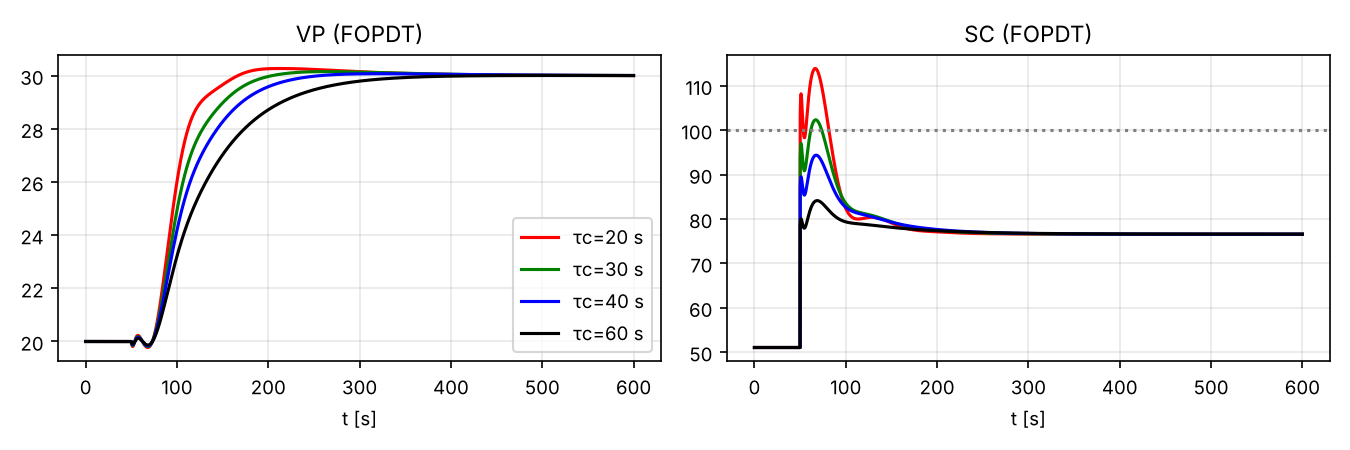
\includegraphics[width=.95\textwidth]{figs/i11_tc.png}\caption{Efeito de $\tau_c$ na VP e no SC (simulação com FOPDT).}\end{figure}
\begin{just}Adoto $\tau_c=40$ s. Com 20 e 30 s o SC da simulação passa de 100\,\% (na bancada o SC saturaria e a simulação linear deixaria de valer). Com 60 s a resposta fica lenta (63,2\,\% em 87 s) sem ganho real. Com 40 s o pico do SC é 94\,\% e o sobressinal é menor que 1\,\%. Além disso $\tau_c=40$ s é maior que o atraso $t_0=25{,}9$ s, o que mantém a malha robusta ao tempo morto. O script do professor usa $\lambda=60$ s (para a planta dele, $\tau=82{,}5$ s); se ele indicar outro valor, basta trocar $\tau_c$ nas fórmulas.\end{just}

\subsection{Cálculo passo a passo ($\tau_c=40$ s)}
\textbf{Passo 1 --- forma real/série (Tabela 7-4.1):}
\[
K_c'=\frac{\tau}{K(t_0+\tau_c)}=\frac{78{,}03}{0{,}3918\,(25{,}92+40)}=\frac{78{,}03}{0{,}3918\cdot65{,}92}=\frac{78{,}03}{25{,}83}=3{,}021\ \%\mathrm{SC}/\%\mathrm{VP},
\]
\[
\tau_I'=\tau=78{,}03\ \mathrm{s},\qquad \tau_D'=\frac{t_0}2=\frac{25{,}92}{2}=12{,}96\ \mathrm{s}.
\]
\textbf{Passo 2 --- conversão para a forma ideal (Seção 7.5):}
\[
K_p=K_c'\Big(1+\frac{\tau_D'}{\tau_I'}\Big)=3{,}021\Big(1+\frac{12{,}96}{78{,}03}\Big)=3{,}021\cdot1{,}1661=3{,}523,
\]
\[
T_i=\tau_I'+\tau_D'=78{,}03+12{,}96=90{,}99\ \mathrm{s},\qquad T_d=\frac{\tau_I'\tau_D'}{\tau_I'+\tau_D'}=\frac{78{,}03\cdot12{,}96}{90{,}99}=\frac{1011{,}2}{90{,}99}=11{,}11\ \mathrm{s}.
\]
\textbf{Conferência com a fórmula direta (script do professor):} $K_p=\dfrac{2\cdot78{,}03+25{,}92}{2\cdot0{,}3918\cdot(40+25{,}92)}=\dfrac{181{,}98}{51{,}66}=3{,}523$ $\checkmark$.

\textbf{Passo 3 --- parâmetros do PI\_D paralelo do OpenPLC:}
\[\begin{gathered}
K_i=\frac{K_p}{T_i}=\frac{3{,}523}{90{,}99}=0{,}03872\ \mathrm{s^{-1}},\\ K_d=K_pT_d=3{,}523\cdot11{,}11=39{,}15\ \mathrm{s},\\ \mu T_d=0{,}1\cdot11{,}11=1{,}11\ \mathrm{s}.
\end{gathered}\]
\begin{res}$K_p=3{,}523$;\quad $K_i=0{,}03872$ (ou $T_i=90{,}99$ s);\quad $K_d=39{,}15$ (ou $T_d=11{,}11$ s);\quad $\mu=0{,}1$.\\
Lei de controle: $SC(t)=K_pe(t)+K_i\!\int e\,dt-K_d\dfrac{d}{dt}VP_{filtrada}(t)$.\end{res}

\subsection{Simulação}
Degrau de SP de 20 para 30\,\% em $t=50$ s, partindo do regime com $SC_0=20/K\approx51{,}0\,\%$ (FOPDT) e $50{,}4\,\%$ (FT completa, $K_3=0{,}3971$). \emph{Comportamento imediato do SC:} em $t=50$ s o termo proporcional dá um salto $K_p\Delta SP=3{,}523\cdot10=35{,}2$ pontos (de 51,0 para $\approx86$\,\%); a derivada não contribui com ``chute'' porque age só sobre a VP.
\begin{figure}[H]\centering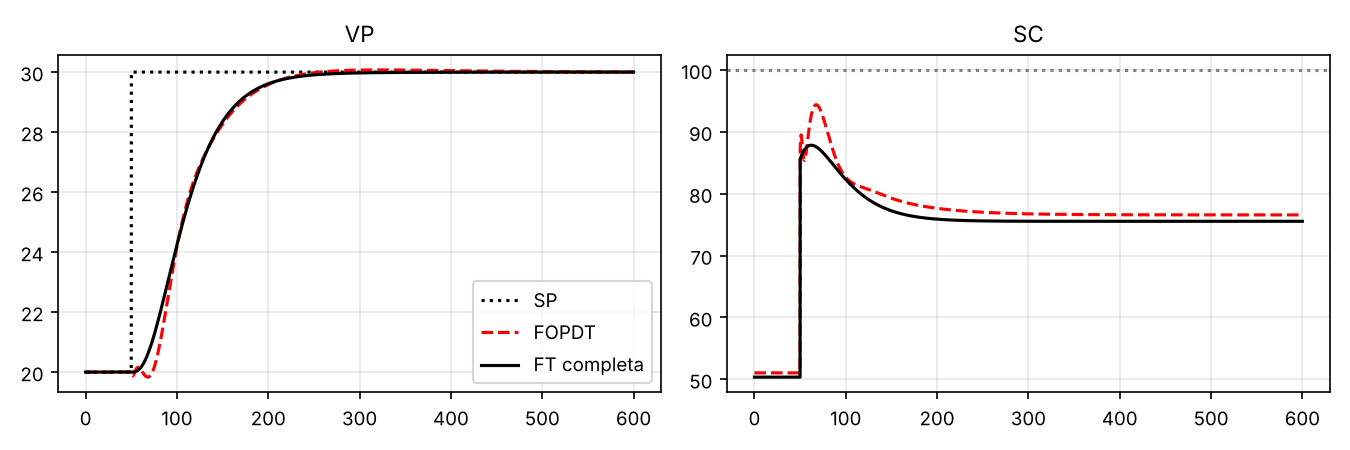
\includegraphics[width=.95\textwidth]{figs/i11.png}\caption{Item 1.1: VP e SC simulados (FOPDT em vermelho tracejado; FT completa em preto).}\end{figure}
\begin{center}\small
\begin{tabular}{lccccc}\toprule & sobress.\ [\%] & $t_{63,2}$ [s] & $t_s$ ($\pm2\%$) [s] & pico do SC [\%] & SC final [\%]\\\midrule
FOPDT & 0,7 & 67,9 & 169,6 & 94,4 & 76,6\\ FT completa & 0,0 & 69,6 & 172,8 & 87,8 & 75,5\\\bottomrule\end{tabular}\end{center}
$SC_{final}=SP_1/K$: $30/0{,}3918=76{,}6$ (FOPDT) e $30/0{,}3971=75{,}5$ (completa); a diferença vem de $K$ ($1{,}3\,\%$).

\textbf{Polos de malha fechada} (raízes de $C_dD_G+C_nN_G$, com Padé de 3ª ordem): FOPDT: $-0{,}511\pm0{,}397j$, $-0{,}0638\pm0{,}0903j$, $-0{,}0182$, $-0{,}0130$; FT completa: $-0{,}902$, $-0{,}0832$, $-0{,}0422$, $-0{,}0351$, $-0{,}0109$. Todos com parte real negativa $\Rightarrow$ malha estável nos dois modelos.

\textbf{Margens da malha aberta $L=(PI+D)G$:} FOPDT: $GM=3{,}7$ (11,4 dB), $PM=78{,}4^\circ$; FT completa: $GM=59{,}7$ (35,5 dB), $PM=81{,}4^\circ$. A margem de fase é praticamente igual nos dois modelos; a margem de ganho da FOPDT é muito menor, como visto na Seção 6.2.
\begin{just}Os dois modelos concordam no formato e na escala de tempo da VP. A FOPDT mostra um pequeno sobressinal e um pico de SC maior (94 contra 88\,\%) porque seu atraso puro e o ganho um pouco diferente alteram a ação proporcional+derivativa.\end{just}
\begin{todo}Procedimento: (i) medir $R$ e $C$ e conferir $K$, $\tau$, $t_0$ pelo degrau em malha aberta; (ii) malha aberta com SO$=20/K\approx50{,}4\,\%$ até $\Vc3\approx20\,\%$; (iii) passar a automático com $SP=VP$ e os parâmetros acima (conferir se o bloco pede $K_p$, $K_i$, $K_d$ ou $K_p$, $T_i$, $T_d$); (iv) aplicar $SP$: 20 $\to$ 30\,\% e gravar SO, SP, VP. Confrontar VP exp.\ $\times$ simulada e SC exp.\ ($=$ SO) $\times$ simulado (figura acima). Resultados: \underline{\hspace{6cm}}\end{todo}

%------------------------------------------------------------------
\section{Item 2.1: PID 2GL (método do $\alpha$ de Juliana Dalmaso)}
\subsection{O que é pedido}
``Uma sintonia do PID 2GL seguindo a mesma metodologia adotada no TCC de Juliana Dalmaso da Silva para escolha do alfa e verifique o sucesso da sintonia confrontando simulação com o experimental quando é aplicado um degrau no SP.''

\subsection{A metodologia do TCC}
Com PID de 1 grau de liberdade, a malha fechada é $VP=\dfrac{PID\,H}{1+PID\,H}SP+\dfrac{H}{1+PID\,H}D$ ($H$ = planta, $D$ = distúrbio). Uma única sintonia não otimiza as duas respostas: a sintonia \emph{servo} (boa para SP) tem ganho menor e a \emph{regulatória} (boa para distúrbio) tem ganho maior, mas ao mudar o SP exige muito do atuador e satura o SC. O PID 2GL resolve isso colocando um filtro no SP:
\begin{formula}
$\displaystyle C_f(s)=\frac{(1-\alpha)T_is+1}{T_is+1},\qquad VP=\frac{C_f\,PI\,G}{1+(PI+D)G}\,SP+\frac{G}{1+(PI+D)G}\,D .$
\end{formula}
\begin{just}$C_f$ aparece \emph{só} na resposta ao SP; a resposta ao distúrbio fica a da sintonia regulatória, qualquer que seja $\alpha$. O filtro é um avanço--atraso. Para ver o efeito, multiplique $C_f$ pelo $PI=K_p\dfrac{T_is+1}{T_is}$: o zero $(T_is+1)$ do PI cancela o polo de $C_f$ e fica $C_f\,PI=K_p\dfrac{(1-\alpha)T_is+1}{T_is}$. Com $\alpha=0$ é o PI\_D comum; com $\alpha\to1$ vira $K_p/(T_is)$, isto é, o SP entra só pela integral (resposta suave, sem salto proporcional no SC).\end{just}
O TCC tem quatro passos: (1) sintonizar o PID para \textbf{controle regulatório} (síntese direta com $\tau_c$ pequeno); (2) sintonizar um PID para \textbf{controle servo} (mesma síntese com $\tau_c$ grande, no TCC $\tau_c=\tau$) e simulá-lo só como \emph{referência} da resposta desejada ao SP; (3) simular o 2GL variando $\alpha$ (no TCC: 0,4; 0,7; 0,99); (4) escolher o $\alpha$ cuja resposta ao SP fica mais próxima da servo, observando que o SC fique menor que o do regulatório (no TCC o $\alpha=0{,}7$ foi o escolhido).

\subsection{Passos 1 e 2: sintonias regulatória e servo}
Mesma fórmula do item 1.1, mudando $\tau_c$. Servo: $\tau_c=\tau=78{,}03$ s. Regulatório: $\tau_c=20$ s (pequeno, mas não menor que o razoável para $t_0=25{,}9$ s; com FOPDT: $GM=2{,}6$, $PM=73^\circ$).
\begin{align*}
\text{servo:}\ K_c'&=\frac{78{,}03}{0{,}3918\,(25{,}92+78{,}03)}=\frac{78{,}03}{0{,}3918\cdot103{,}95}=\frac{78{,}03}{40{,}73}=1{,}916\\ &\Rightarrow K_p=1{,}916\cdot1{,}1661=2{,}234\\
\text{regulatório:}\ K_c'&=\frac{78{,}03}{0{,}3918\,(25{,}92+20)}=\frac{78{,}03}{0{,}3918\cdot45{,}92}=\frac{78{,}03}{17{,}99}=4{,}337\\ &\Rightarrow K_p=4{,}337\cdot1{,}1661=5{,}057
\end{align*}
Nos dois casos $T_i=90{,}99$ s e $T_d=11{,}11$ s (não dependem de $\tau_c$). Regulatório: $K_i=5{,}057/90{,}99=0{,}05558$, $K_d=5{,}057\cdot11{,}11=56{,}21$. Servo: $K_i=2{,}234/90{,}99=0{,}02455$, $K_d=2{,}234\cdot11{,}11=24{,}83$. Como esperado pelo TCC, \textbf{o ganho do regulatório ($K_p=5{,}06$) é maior que o do servo ($2{,}23$).}

\subsection{Passos 3 e 4: escolha do $\alpha$}
Simulei o 2GL (regulatório + $C_f$) com $\alpha=0{,}4$; $0{,}7$; $0{,}99$ (valores do TCC) e fiz também uma varredura de $\alpha$ de 0 a 0,99 em passos de 0,01, medindo o erro RMS entre a VP do 2GL e a VP servo (referência) em $50<t<550$ s, em \% do degrau:
\[
\varepsilon(\alpha)=\frac{100}{\Delta SP}\sqrt{\frac1N\sum_k\big(VP_{2GL}(t_k;\alpha)-VP_{servo}(t_k)\big)^2},\qquad \Delta SP=10\,\%.
\]
\begin{figure}[H]\centering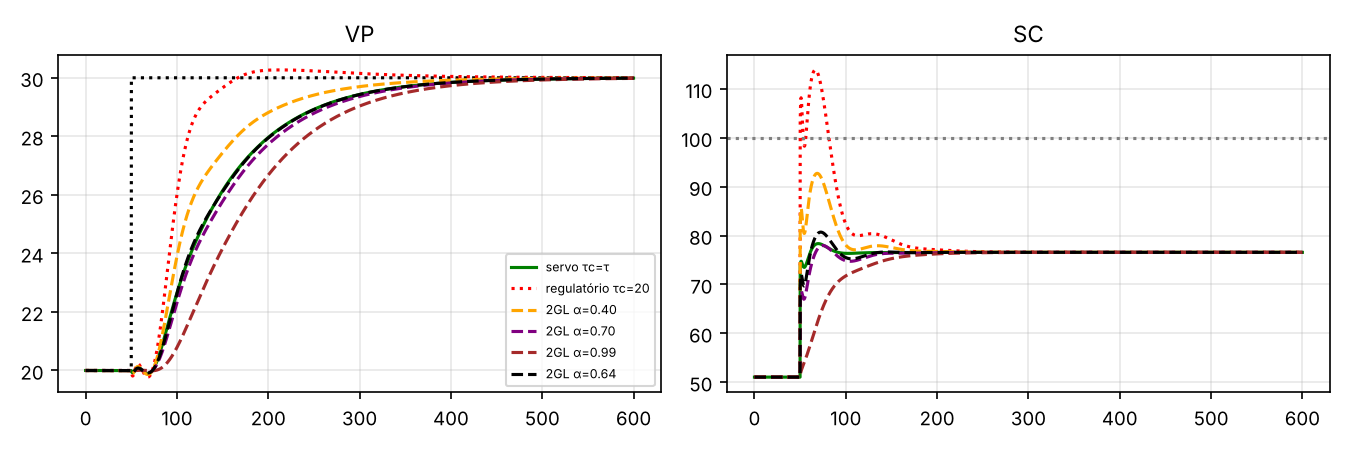
\includegraphics[width=.95\textwidth]{figs/i21.png}\caption{Item 2.1: PI\_D servo (verde), regulatório (vermelho pontilhado) e 2GL para $\alpha=0{,}4$; $0{,}7$; $0{,}99$ e $0{,}64$ (preto). Simulação com FOPDT.}\end{figure}
\begin{figure}[H]\centering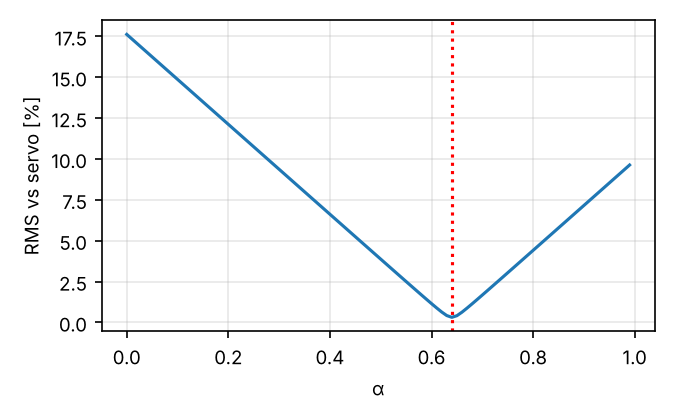
\includegraphics[width=.5\textwidth]{figs/i21_alpha.png}\caption{Erro RMS entre a VP do 2GL e a VP servo em função de $\alpha$.}\end{figure}
\begin{center}\small
\begin{tabular}{lcccc}\toprule Caso (FOPDT) & sobress.\ [\%] & $t_{63,2}$ [s] & pico do SC [\%] & RMS $\times$ servo [\%]\\\midrule
PI\_D servo ($\tau_c=\tau$) & 0,0 & 104 & 78 & (referência)\\
PI\_D regulatório ($\tau_c=20$) & 2,7 & 51,5 & 114 & 17,6\\
2GL $\alpha=0{,}40$ & 0,0 & 74,4 & 92,7 & 6,62\\
2GL $\alpha=0{,}70$ & 0,0 & 111,4 & 78,0 & 1,67\\
2GL $\alpha=0{,}99$ & 0,0 & 141,3 & 76,6 & 9,63\\
\textbf{2GL $\alpha=0{,}64$} & 0,0 & 104,5 & 80,7 & \textbf{0,31}\\\bottomrule\end{tabular}\end{center}
O mínimo ocorre em $\alpha=0{,}64$ com $\varepsilon=0{,}31\,\%$.
\begin{just}$\alpha=0{,}4$ ainda é rápido demais (RMS 6,6\,\%) e o SC chega a 93\,\%; $\alpha=0{,}99$ é lento demais (RMS 9,6\,\%, $t_{63}=141$ s). O valor $\alpha=0{,}7$ do TCC dá RMS 1,7\,\% e funciona, mas a varredura mostra que $\alpha=0{,}64$ reproduz ainda melhor a resposta servo (RMS 0,31\,\%), porque o $\alpha$ ótimo depende da planta (aqui, FOPDT com atraso; no TCC era um processo de 1ª ordem sem atraso). Adoto $\alpha=0{,}64$, mantendo a mesma metodologia do TCC (escolha por simulação do $\alpha$ que aproxima o servo, com SC menor que o do regulatório: pico de 81\,\% contra 114\,\%, que satura).\end{just}
Com a FT completa: $t_{63}=102{,}6$ s e pico do SC de 75,5\,\%.

\subsection{Parâmetros finais para o OpenPLC (PI\_D2GL)}
\begin{res}$K_p=5{,}057$;\quad $K_i=0{,}05558\ \mathrm{s^{-1}}$ ($T_i=90{,}99$ s);\quad $K_d=56{,}21$ ($T_d=11{,}11$ s);\quad $\mu=0{,}1$;\quad $\alpha=0{,}64$ (filtro do SP com $\beta=1$ fixo, como no CLP Omron do TCC).\end{res}
\begin{todo}Passar a automático com $SP=VP$ e os parâmetros acima; aplicar degrau de SP 20 $\to$ 30\,\%; gravar SO, SP, VP. Confrontar VP e SC com a simulação (FOPDT e FT completa). Se possível repetir com $\alpha=0$ (PI\_D regulatório comum) para mostrar o efeito de $\alpha$ (SC chegando a 114\,\%, isto é, saturando). Resultados: \underline{\hspace{6cm}}\end{todo}

%------------------------------------------------------------------
\section{Item 3.1: integral do erro mínimo (seção 7-2.3)}
\subsection{O método}
Na seção 7-2.3 o livro apresenta correlações que minimizam um índice de integral do erro, aqui $\mathrm{IAE}=\int_0^\infty|e|\,dt$, para plantas FOPDT. Para o PID ideal, com $r=t_0/\tau$ (válido para $0{,}1<r<1$):
\begin{formula}
\textbf{Tabela 7-2.3 (ponto fixo, Rovira):}\quad $K_c=\dfrac{1{,}086}{K}\,r^{-0{,}869},\quad \tau_I=\dfrac{\tau}{0{,}740-0{,}130\,r},\quad \tau_D=0{,}348\,\tau\,r^{0{,}914}$.\\[3pt]
\textbf{Tabela 7-2.2 (distúrbio, López):}\quad $K_c=\dfrac{1{,}435}{K}\,r^{-0{,}921},\quad \tau_I=\dfrac{\tau}{0{,}878}\,r^{0{,}749},\quad \tau_D=0{,}482\,\tau\,r^{1{,}137}$.
\end{formula}
\begin{just}Como o experimento é um degrau no SP (como nos outros itens), a sintonia principal é a da Tabela 7-2.3 (ponto fixo); calculo também a de distúrbio para comparar. Aqui $r=25{,}92/78{,}03=0{,}3322$, dentro da faixa de validade. As tabelas já fornecem o PID na forma ideal (paralela), então \textbf{não há conversão série$\to$ideal}: $K_p=K_c$, $K_i=K_c/\tau_I$, $K_d=K_c\tau_D$.\end{just}

\subsection{Cálculo passo a passo}
Potências calculadas por logaritmo: $\ln r=\ln0{,}3322=-1{,}1021$.

\textbf{Ponto fixo (Tabela 7-2.3):}
\begin{align*}
r^{-0{,}869}&=e^{-0{,}869\cdot(-1{,}1021)}=e^{0{,}9577}=2{,}606\\
\frac{1{,}086}{K}&=\frac{1{,}086}{0{,}3918}=2{,}772\\
K_p&=2{,}772\cdot2{,}606=\mathbf{7{,}222}\\
T_i&=\frac{78{,}03}{0{,}740-0{,}130\cdot0{,}3322}=\frac{78{,}03}{0{,}740-0{,}0432}=\frac{78{,}03}{0{,}6968}=\mathbf{111{,}98\ s}\\
r^{0{,}914}&=e^{0{,}914\cdot(-1{,}1021)}=e^{-1{,}0073}=0{,}3652\\T_d&=0{,}348\cdot78{,}03\cdot0{,}3652=27{,}15\cdot0{,}3652=\mathbf{9{,}92\ s}\\
K_i&=\frac{K_p}{T_i}=\frac{7{,}222}{111{,}98}=\mathbf{0{,}06449}\\K_d&=K_pT_d=7{,}222\cdot9{,}917=\mathbf{71{,}63}
\end{align*}
\textbf{Distúrbio (Tabela 7-2.2), para comparar:}
\begin{align*}
r^{-0{,}921}&=e^{1{,}0150}=2{,}759\\K_p&=\frac{1{,}435}{0{,}3918}\cdot2{,}759=3{,}663\cdot2{,}759=10{,}11\\
r^{0{,}749}&=e^{-0{,}8254}=0{,}4380\\T_i&=\frac{78{,}03}{0{,}878}\cdot0{,}4380=38{,}93\ \mathrm{s}\\
r^{1{,}137}&=e^{-1{,}2531}=0{,}2856\\T_d&=0{,}482\cdot78{,}03\cdot0{,}2856=10{,}74\ \mathrm{s}\\
K_i&=10{,}11/38{,}93=0{,}2596\\K_d&=10{,}11\cdot10{,}74=108{,}6
\end{align*}
\begin{res}Ponto fixo: $K_p=7{,}222$; $K_i=0{,}06449$ ($T_i=111{,}98$ s); $K_d=71{,}63$ ($T_d=9{,}92$ s); $\mu=0{,}1$.\end{res}

\subsection{Simulação}
Degrau de SP de 20 para 25\,\% em $t=50$ s (menor que nos outros itens porque o ganho alto desta sintonia faria o SC passar de 100\,\% com 20 $\to$ 30\,\%).
\begin{figure}[H]\centering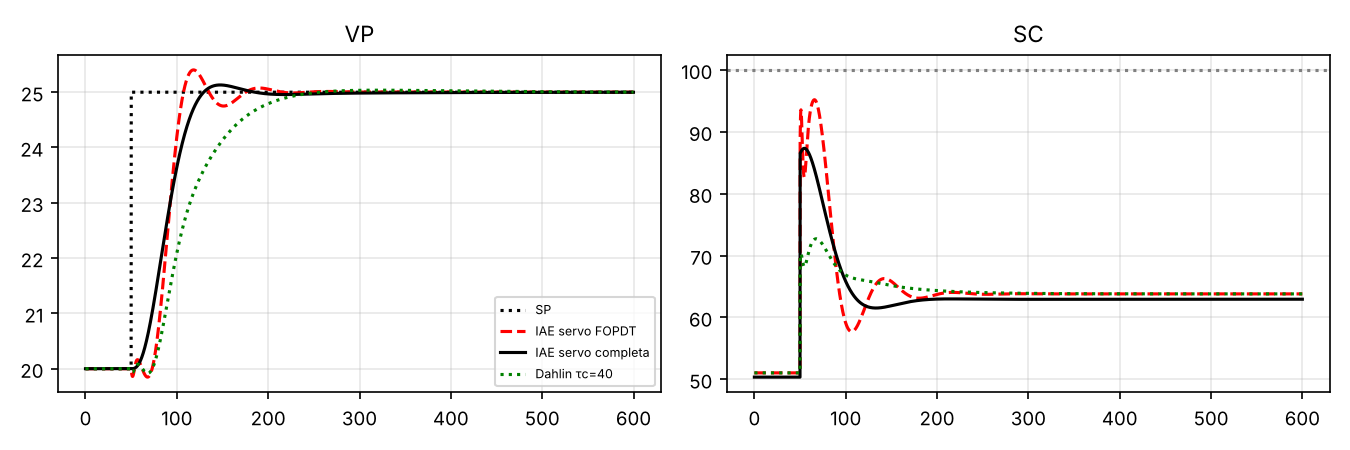
\includegraphics[width=.95\textwidth]{figs/i31.png}\caption{Item 3.1: IAE ponto fixo (FOPDT tracejado vermelho; FT completa preto) e Dahlin $\tau_c=40$ s do item 1.1 (verde pontilhado), degrau 20 $\to$ 25\,\%.}\end{figure}
\begin{center}\small
\begin{tabular}{lcccc}\toprule Sintonia (20 $\to$ 25\,\%), FOPDT / completa & sobress.\ [\%] & $t_{63,2}$ [s] & $t_s$ [s] & pico do SC [\%]\\\midrule
IAE ponto fixo (7-2.3) & 8,1 / 2,6 & 43,7 / 44,4 & 117 / 110 & 95 / 87\\
IAE distúrbio (7-2.2) & 83,6 / 42,3 & 37,8 / 33,3 & 227 / 201 & 129 / 107\\
Dahlin $\tau_c=40$ s (item 1.1) & 0,7 / 0,0 & 67,9 / 69,6 & 170 / 173 & 73 / 69\\\bottomrule\end{tabular}\end{center}
Margens da malha aberta com a sintonia de ponto fixo: FOPDT $GM=1{,}9$, $PM=64^\circ$; FT completa $GM=32{,}0$, $PM=71^\circ$.
\begin{just}A sintonia de ponto fixo é a mais rápida ($t_{63}=44$ s contra 68 s do Dahlin), à custa de sobressinal maior (8,1\,\% na FOPDT, 2,6\,\% na completa) e de $K_p$ mais alto --- esperado de um método que minimiza o erro integral sem penalizar o esforço de controle. A sintonia de distúrbio é ainda mais agressiva e, aplicada a um degrau de SP, produz sobressinal de 84\,\% na FOPDT: foi projetada para rejeitar distúrbios, não para seguir SP (a ideia do TCC: servo e regulatório exigem sintonias diferentes). A diferença de sobressinal entre FOPDT e completa vem do atraso puro da FOPDT, que reduz a margem de ganho (1,9 contra 32).\end{just}
\begin{todo}Mesmo procedimento do item 1.1 com $K_p=7{,}222$, $K_i=0{,}06449$, $K_d=71{,}63$, $\mu=0{,}1$ e degrau de SP 20 $\to$ 25\,\%. Confrontar VP e SC com a figura. Resultados: \underline{\hspace{6cm}}\end{todo}

%------------------------------------------------------------------
\section{Item 4.1: Ziegler--Nichols de razão de decaimento 1/4 (Tabela 7-1.1)}
\subsection{O método}
A Tabela 7-1.1 usa o \textbf{ganho final} $K_{cu}$ e o \textbf{período final} $T_u$: com controle só proporcional, aumenta-se $K_c$ até a VP oscilar com amplitude constante; $K_{cu}$ é esse ganho e $T_u$ o período da oscilação. Para o PID (forma real/série), razão de decaimento 1/4 (cada pico é 1/4 do anterior):
\begin{formula}$K_c'=\dfrac{K_{cu}}{1{,}7},\qquad\tau_I'=\dfrac{T_u}{2},\qquad\tau_D'=\dfrac{T_u}{8}$, convertidos à forma ideal pela Seção 7.5.\end{formula}
\subsection{$K_{cu}$ e $T_u$}
Experimentalmente serão medidos na bancada (teste de ganho final). Para poder simular, calculo-os da FT completa de $\Vc3$ pelo critério de Routh (Seção 6.2): $K_{cu}=38{,}97$, $\omega_u=0{,}09125$ rad/s, $T_u=68{,}85$ s. Confirmação pelos polos de $1+K_cG(s)=0$:
\begin{center}\small\begin{tabular}{ccc}\toprule $K_c$ & polos complexos dominantes & comportamento\\\midrule
$0{,}5K_{cu}=19{,}5$ & $-0{,}0108\pm0{,}0702j$ & oscilação amortece\\
$K_{cu}=39{,}0$ & $\approx0\pm0{,}0913j$ & oscilação sustentada, $T_u=2\pi/0{,}0913=68{,}85$ s\\
$1{,}2K_{cu}=46{,}8$ & $+0{,}0033\pm0{,}0975j$ & oscilação cresce (instável)\\\bottomrule\end{tabular}\end{center}
\begin{figure}[H]\centering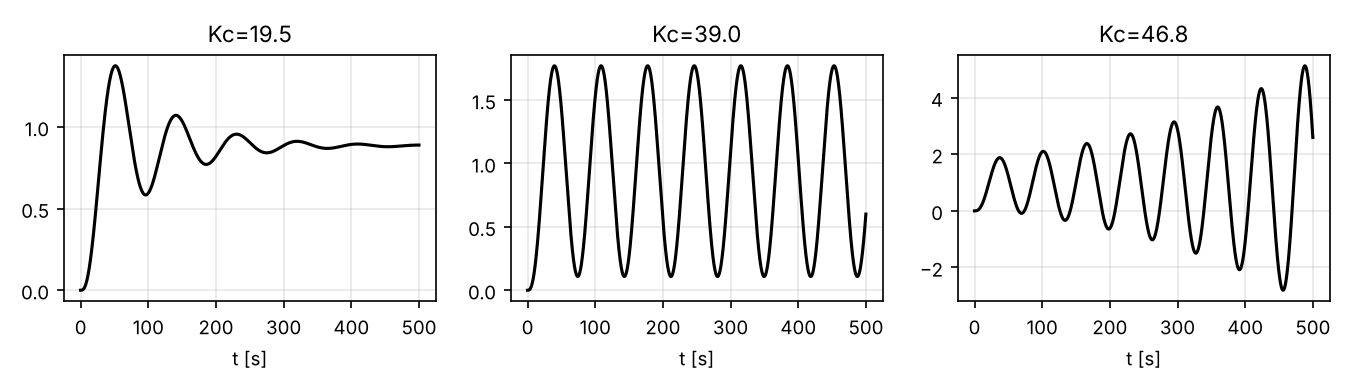
\includegraphics[width=.95\textwidth]{figs/i41_kcu.png}\caption{Teste de ganho final simulado (FT completa, $K_c$ puro, degrau no SP).}\end{figure}
\begin{just}Uso a FT \emph{completa} (e não a reduzida) para obter $K_{cu}$ e $T_u$ porque o método de Ziegler--Nichols exige o comportamento real da planta no limite de estabilidade. A FOPDT daria $K_{cu}=13{,}7$ e $T_u=92{,}7$ s, bem diferentes do real (39,0 e 68,9 s). Na bancada a oscilação sustentada será limitada pela saturação do SC em 0--100\,\%; deve-se registrar o menor $K_c$ que sustenta a oscilação e o período $T_u$ medido, e recalcular os parâmetros com as mesmas fórmulas abaixo.\end{just}

\subsection{Cálculo passo a passo}
\textbf{Passo 1 --- forma real/série:}
\[
K_c'=\frac{K_{cu}}{1{,}7}=\frac{38{,}97}{1{,}7}=22{,}92,\qquad\tau_I'=\frac{T_u}2=\frac{68{,}85}{2}=34{,}43\ \mathrm{s},\qquad\tau_D'=\frac{T_u}8=\frac{68{,}85}{8}=8{,}607\ \mathrm{s}.
\]
\textbf{Passo 2 --- forma ideal (Seção 7.5):}
\[
K_p=K_c'\Big(1+\frac{\tau_D'}{\tau_I'}\Big)=22{,}92\Big(1+\frac{8{,}607}{34{,}43}\Big)=22{,}92\cdot1{,}25=28{,}65,
\]
\[
T_i=\tau_I'+\tau_D'=34{,}43+8{,}607=43{,}03\ \mathrm{s},\qquad T_d=\frac{34{,}43\cdot8{,}607}{43{,}03}=\frac{296{,}3}{43{,}03}=6{,}885\ \mathrm{s}.
\]
\emph{Conferência por fórmula direta:} como $\tau_D'/\tau_I'=1/4$ sempre, $K_p=1{,}25\,K_{cu}/1{,}7=0{,}735K_{cu}=28{,}65$, $T_i=\frac58T_u=43{,}03$ s e $T_d=\frac1{10}T_u=6{,}885$ s $\checkmark$.

\textbf{Passo 3 --- OpenPLC:}
\[
K_i=\frac{K_p}{T_i}=\frac{28{,}65}{43{,}03}=0{,}6659\ \mathrm{s^{-1}},\qquad K_d=K_pT_d=28{,}65\cdot6{,}885=197{,}3\ \mathrm{s},\qquad\mu=0{,}1 .
\]
O ganho em alta frequência do PID (com o filtro $\mu=0{,}1$) é $K_p(1+1/\mu)=28{,}65\cdot11\approx315$: controlador de ganho alto, sensível a ruído de medição (a quantização do ADC é 0,098\,\%).
\begin{res}$K_p=28{,}65$;\ $K_i=0{,}6659$ ($T_i=43{,}03$ s);\ $K_d=197{,}3$ ($T_d=6{,}885$ s);\ $\mu=0{,}1$.\end{res}

\subsection{Simulação}
Degrau de SP de 10 para 12\,\% em $t=50$ s (pequeno porque o ganho alto faria o SC saturar em degraus maiores); $SC_0=10/0{,}3971=25{,}2\,\%$.
\begin{figure}[H]\centering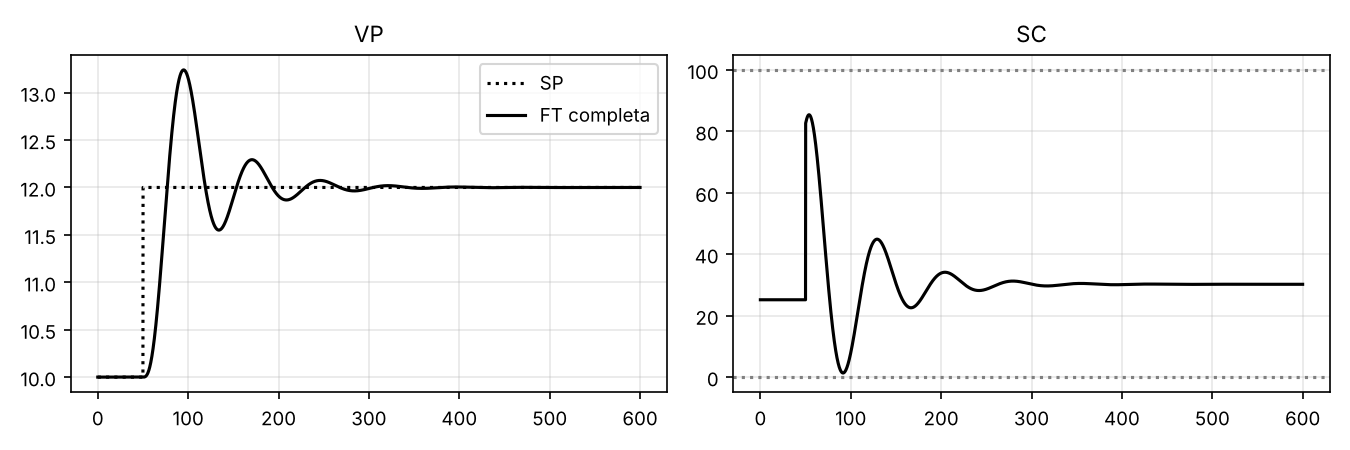
\includegraphics[width=.95\textwidth]{figs/i41.png}\caption{Item 4.1: PID de Ziegler--Nichols simulado com a FT completa.}\end{figure}
\begin{center}\small\begin{tabular}{lccccc}\toprule & sobress.\ [\%] & $t_{63,2}$ [s] & $t_s$ [s] & pico do SC [\%] & $GM$ / $PM$\\\midrule FT completa & 62 & 21 & 209 & 85 & 7,8 / 22$^\circ$\\\bottomrule\end{tabular}\end{center}
\textbf{Razão de decaimento.} Na simulação o 1º excesso acima do SP final é $1{,}24\,\%$ e o 2º é $0{,}29\,\%$ (instantes 95 s e 171 s): razão $=0{,}293/1{,}24=0{,}236\approx1/4$, que é o critério de projeto do método.

\textbf{Por que não simular com a FOPDT.} Os polos de malha fechada da FOPDT com esta sintonia têm parte real positiva ($+0{,}027\pm0{,}087j$ s$^{-1}$): a malha é \emph{instável}, porque $K_c'=22{,}9$ e $K_p=28{,}7$ são maiores que o ganho final da FOPDT ($K_{cu,red}=13{,}7$). Com a FT completa, todos os polos de malha fechada têm parte real negativa (o maior é $-0{,}0176$).
\begin{figure}[H]\centering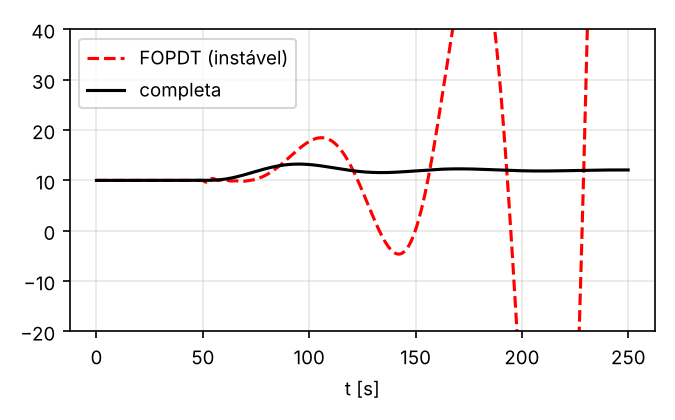
\includegraphics[width=.5\textwidth]{figs/i41_unst.png}\caption{O mesmo PID aplicado à FOPDT (instável) e à FT completa.}\end{figure}
\begin{just}A sintonia de Z--N foi \emph{projetada} para uma planta real em que se mediu $K_{cu}$ e $T_u$; o modelo FOPDT, ao trocar 3 polos por 1 polo e atraso, tem margem de ganho menor, então a sintonia que é estável na planta completa torna a FOPDT instável. Os parâmetros de Z--N só são válidos com $K_{cu}$ e $T_u$ da planta real. A resposta tem sobressinal grande (62\,\% do degrau), característico da razão 1/4; o SC chega a tocar o limite inferior no primeiro retorno, o que na bancada produzirá saturação e leve diferença em relação à simulação linear.\end{just}
\begin{todo}(i) Teste de ganho final: apenas $K_p$ ($K_i=K_d=0$), aumentar até oscilação sustentada, anotar $K_{cu}$ e $T_u$ (esperado: Figura do teste acima); (ii) recalcular os parâmetros com as fórmulas acima e implementar $K_p$, $K_i$, $K_d$, $\mu=0{,}1$; (iii) degrau de SP 10 $\to$ 12\,\%, gravar SO, SP, VP; (iv) confrontar VP e SC com a figura de simulação acima. Resultados: \underline{\hspace{6cm}}\end{todo}

%------------------------------------------------------------------
\section{Resumo dos controladores (para o OpenPLC)}
\begin{center}\small
\begin{tabular}{lccccc}\toprule Sintonia & $K_p$ & $T_i$ [s] & $T_d$ [s] & $K_i=K_p/T_i$ & $K_d=K_pT_d$\\\midrule
1.1 Dahlin ($\tau_c=40$ s) & 3,523 & 90,99 & 11,11 & 0,03872 & 39,15\\
2.1 PI\_D2GL (regulatório $\tau_c=20$ s, $\alpha=0{,}64$) & 5,057 & 90,99 & 11,11 & 0,05558 & 56,21\\
3.1 IAE ponto fixo (7-2.3) & 7,222 & 111,98 & 9,92 & 0,06449 & 71,63\\
4.1 Ziegler--Nichols (7-1.1) & 28,65 & 43,03 & 6,885 & 0,6659 & 197,3\\\bottomrule\end{tabular}\end{center}
Todos com $\mu=0{,}1$ (filtro derivativo $\mu T_d$), derivada na VP, $T_i$ e $T_d$ em segundos e $K_p$ em \%SC/\%VP.

\section{Conclusões}
\begin{itemize}
\item As FTs completas, deduzidas das equações dos nós com os $R$ e $C$ medidos, têm três polos reais ($\tau=68{,}7$; $16{,}0$; $10{,}4$ s) e reproduzem o degrau experimental com RMS de 0,7--1,7\,\% do degrau.
\item $\Vc1$ é curva tipo C ($\tau=23{,}3$ s, sem atraso); $\Vc2$ e $\Vc3$ são tipo S (Smith: $\Vc3$: $K=0{,}392$, $\tau=78{,}0$ s, $t_0=25{,}9$ s).
\item A FOPDT mantém a margem de fase da malha aberta (diferenças de até $6^\circ$ para $K_c\le5$) e subestima a margem de ganho (é conservadora). Por isso as sintonias dos itens 1.1, 2.1 e 3.1 são calculadas com a FOPDT (como pede o enunciado), enquanto $K_{cu}$ e $T_u$ do item 4.1 devem vir da planta real.
\item Os quatro controladores foram simulados (VP e SC, FOPDT e FT completa); as comparações com o experimento, VP e SC, serão feitas após os ensaios na bancada (assim como os itens 1.2, 1.3, 2.2 e 4.2).
\end{itemize}
